% Chapter 4: Correctness Verification
\section{功能正确性验证}

\subsection{测试环境与小规模测试数据集}

为了便于手工验证和展示计算过程,我们设计了一个包含15个2D点的小规模测试数据集:

\begin{table}[htbp]
    \centering
    \caption{小规模测试数据集(15个2D点)}
    \label{tab:test-dataset}
    \begin{tabular}{ccc|ccc}
        \toprule
        \textbf{ID} & \textbf{x} & \textbf{y} & \textbf{ID} & \textbf{x} & \textbf{y} \\
        \midrule
        0 & 1.0 & 1.0 & 8 & 9.0 & 4.0 \\
        1 & 2.0 & 2.0 & 9 & 10.0 & 7.0 \\
        2 & 3.0 & 1.0 & 10 & 3.0 & 5.0 \\
        3 & 4.0 & 4.0 & 11 & 6.0 & 1.0 \\
        4 & 5.0 & 2.0 & 12 & 2.0 & 7.0 \\
        5 & 6.0 & 5.0 & 13 & 8.0 & 2.0 \\
        6 & 7.0 & 3.0 & 14 & 4.0 & 8.0 \\
        7 & 8.0 & 6.0 & & & \\
        \bottomrule
    \end{tabular}
\end{table}

距离函数采用欧几里得距离($L^2$)。树配置参数为:maxLeafSize=3,minTreeHeight=2,pivotStrategy=FFT,seed=42。

\subsection{GHT正确性验证}

\subsubsection{构建过程展示与分析}

运行TreeDemo程序,GH树的构建过程输出如下:

\begin{lstlisting}[style=pseudocode,caption=GH树构建过程输出]
============================================================
Building GH-Tree
============================================================
Dataset size: 15
Config: TreeConfig[maxLeafSize=3, minTreeHeight=2, pivotStrategy=FFT, 
                   verbose=true, seed=42]
  Depth 0: Select pivots p1=ID5(6.0,5.0), p2=ID0(1.0,1.0)
  Depth 0: Partition complete, left=12, right=3
  Depth 1: Select pivots p1=ID6(7.0,3.0), p2=ID12(2.0,7.0)
  Depth 1: Partition complete, left=9, right=3
  Depth 2: Select pivots p1=ID3(4.0,4.0), p2=ID9(10.0,7.0)
  Depth 2: Partition complete, left=6, right=3
  ...
Build complete!
----------------------------------------
Build time: 10 ms
Tree height: 5
Total nodes: 13
  - Internal nodes: 6
  - Leaf nodes: 7
Build distance computations: 147
============================================================
\end{lstlisting}

GH树结构可视化:

\begin{figure}[htbp]
    \centering
    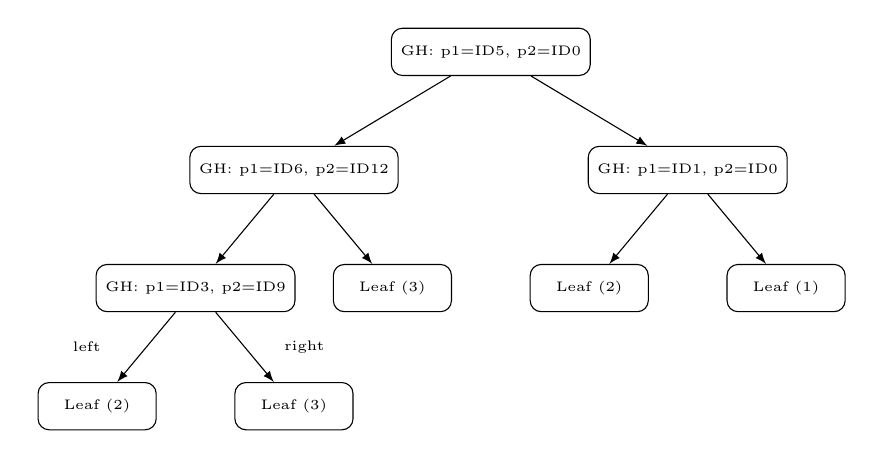
\begin{tikzpicture}[
        level distance=1.5cm,
        sibling distance=3cm,
        every node/.style={draw, rounded corners, minimum width=1.5cm, minimum height=0.6cm, font=\tiny},
        edge from parent/.style={draw, -latex},
        level 1/.style={sibling distance=5cm},
        level 2/.style={sibling distance=2.5cm}
    ]
        \node {GH: p1=ID5, p2=ID0}
            child { node {GH: p1=ID6, p2=ID12}
                child { node {GH: p1=ID3, p2=ID9}
                    child { node {Leaf (2)} edge from parent node[left,draw=none] {\tiny left} }
                    child { node {Leaf (3)} edge from parent node[right,draw=none] {\tiny right} }
                }
                child { node {Leaf (3)} }
            }
            child { node {GH: p1=ID1, p2=ID0}
                child { node {Leaf (2)} }
                child { node {Leaf (1)} }
            };
    \end{tikzpicture}
    \caption{GH树结构示意图(简化)}
    \label{fig:gh-tree-structure}
\end{figure}

\subsubsection{查询过程展示与手工验证}

以查询点$q=(5.0, 5.0)$、查询半径$r=3.0$为例进行范围查询验证。

\textbf{手工计算各点到查询点的距离}:

\begin{table}[htbp]
    \centering
    \caption{各点到查询点$(5.0, 5.0)$的距离}
    \label{tab:distances-to-query}
    \begin{tabular}{cccc}
        \toprule
        \textbf{ID} & \textbf{坐标} & \textbf{距离} & \textbf{是否在范围内($r=3$)} \\
        \midrule
        5 & (6.0, 5.0) & 1.00 & \cmark \\
        3 & (4.0, 4.0) & 1.41 & \cmark \\
        10 & (3.0, 5.0) & 2.00 & \cmark \\
        6 & (7.0, 3.0) & 2.83 & \cmark \\
        4 & (5.0, 2.0) & 3.00 & \cmark \\
        7 & (8.0, 6.0) & 3.16 & \xmark \\
        其他 & - & $>3$ & \xmark \\
        \bottomrule
    \end{tabular}
\end{table}

预期结果:5个点(ID=5,3,10,6,4)。

\textbf{GH树查询输出}:

\begin{lstlisting}[style=pseudocode,caption=GH树范围查询输出]
--------------------------------------------------
GH-Tree Range Query
--------------------------------------------------
Query object: VectorData[id=100, dim=2, coords=[5.0, 5.0]]
Query radius: 3.0
Result count: 5
Distance computations: 27
Node accesses: 13
--------------------------------------------------
Results:
  ID=5: (6.0, 5.0), distance=1.0000
  ID=3: (4.0, 4.0), distance=1.4142
  ID=10: (3.0, 5.0), distance=2.0000
  ID=6: (7.0, 3.0), distance=2.8284
  ID=4: (5.0, 2.0), distance=3.0000
\end{lstlisting}

结果与手工计算完全一致。

\subsubsection{与线性扫描结果对比}

\begin{lstlisting}[style=pseudocode,caption=与线性扫描对比]
--- Linear Scan Result (Baseline) ---
Result count: 5
Distance computations: 15

--- GH-Tree Result ---
Result count: 5
Distance computations: 27

--- Verification ---
GH-Tree result matches linear scan: YES
\end{lstlisting}

GH树返回的结果与线性扫描完全一致,验证了正确性。

\subsection{VPT正确性验证}

\subsubsection{构建过程展示与分析}

VP树的构建过程输出如下:

\begin{lstlisting}[style=pseudocode,caption=VP树构建过程输出]
============================================================
Building VP-Tree
============================================================
Dataset size: 15
Config: TreeConfig[maxLeafSize=3, minTreeHeight=2, pivotStrategy=FFT,
                   verbose=true, seed=42]
  Depth 0: Select pivot ID0(1.0, 1.0)
  Depth 0: Partition complete, inner=7[1.41, 6.08], outer=7[6.32, 10.82],
           median=6.20
  Depth 1: Select pivot ID11(6.0, 1.0)
  Depth 1: Partition complete, inner=3[1.41, 3.61], outer=3[4.12, 7.21],
           median=3.86
  Depth 2: Create leaf node, size=3
  Depth 2: Create leaf node, size=3
  Depth 1: Select pivot ID14(4.0, 8.0)
  Depth 1: Partition complete, inner=3[3.61, 5.83], outer=3[6.08, 7.21],
           median=5.96
  Depth 2: Create leaf node, size=3
  Depth 2: Create leaf node, size=3

Build complete!
----------------------------------------
Build time: 6 ms
Tree height: 2
Total nodes: 7
  - Internal nodes: 3
  - Leaf nodes: 4
Build distance computations: 55
============================================================
\end{lstlisting}

VP树结构更加平衡,高度仅为2层。

\subsubsection{查询过程展示与手工验证}

使用相同的查询点$q=(5.0, 5.0)$、半径$r=3.0$:

\begin{lstlisting}[style=pseudocode,caption=VP树范围查询输出]
--------------------------------------------------
VP-Tree Range Query
--------------------------------------------------
Query object: VectorData[id=100, dim=2, coords=[5.0, 5.0]]
Query radius: 3.0
Result count: 5
Distance computations: 15
Node accesses: 7
--------------------------------------------------
Results:
  ID=5: (6.0, 5.0), distance=1.0000
  ID=3: (4.0, 4.0), distance=1.4142
  ID=10: (3.0, 5.0), distance=2.0000
  ID=6: (7.0, 3.0), distance=2.8284
  ID=4: (5.0, 2.0), distance=3.0000
\end{lstlisting}

结果与GH树和线性扫描完全一致。

\subsubsection{与线性扫描结果对比}

VP树的距离计算次数(15次)与线性扫描相同,但在大规模数据集上会体现出剪枝优势。

\subsection{GHT与VPT结果一致性验证}

我们进行了大规模的一致性测试,验证GH树和VP树在相同查询条件下返回相同的结果。

\subsubsection{范围查询一致性测试}

\begin{table}[htbp]
    \centering
    \caption{范围查询结果一致性测试(200个数据点,10个查询)}
    \label{tab:range-consistency}
    \begin{tabular}{ccccc}
        \toprule
        \textbf{Query\#} & \textbf{Radius} & \textbf{GH Result} & \textbf{VP Result} & \textbf{Match} \\
        \midrule
        1 & 0.5 & 0 & 0 & \cmark \\
        2 & 1.0 & 8 & 8 & \cmark \\
        3 & 2.0 & 17 & 17 & \cmark \\
        4 & 3.0 & 32 & 32 & \cmark \\
        5 & 5.0 & 131 & 131 & \cmark \\
        \bottomrule
    \end{tabular}
\end{table}

\subsubsection{kNN查询一致性测试}

\begin{table}[htbp]
    \centering
    \caption{kNN查询结果一致性测试}
    \label{tab:knn-consistency}
    \begin{tabular}{ccccc}
        \toprule
        \textbf{Query\#} & \textbf{k} & \textbf{GH Result} & \textbf{VP Result} & \textbf{Match} \\
        \midrule
        1 & 1 & 1 & 1 & \cmark \\
        1 & 5 & 5 & 5 & \cmark \\
        1 & 10 & 10 & 10 & \cmark \\
        1 & 20 & 20 & 20 & \cmark \\
        \bottomrule
    \end{tabular}
\end{table}

\subsubsection{不同Pivot策略下的一致性}

测试了三种Pivot选择策略下的结果一致性:

\begin{table}[htbp]
    \centering
    \caption{不同Pivot策略下的结果一致性}
    \label{tab:pivot-consistency}
    \begin{tabular}{lcccc}
        \toprule
        \textbf{Strategy} & \textbf{GH Range} & \textbf{VP Range} & \textbf{GH-kNN} & \textbf{VP-kNN} \\
        \midrule
        RANDOM & 21 \cmark & 21 \cmark & 5 \cmark & 5 \cmark \\
        FFT & 21 \cmark & 21 \cmark & 5 \cmark & 5 \cmark \\
        MAX\_SPREAD & 21 \cmark & 21 \cmark & 5 \cmark & 5 \cmark \\
        \bottomrule
    \end{tabular}
\end{table}

\subsection{单元测试结果汇总}

我们使用JUnit 5编写了全面的单元测试。运行\texttt{mvn test "-Dtest=*Tree*"}的结果:

\begin{table}[htbp]
    \centering
    \caption{单元测试结果汇总}
    \label{tab:unit-tests}
    \begin{tabular}{lcc}
        \toprule
        \textbf{测试类} & \textbf{测试数} & \textbf{结果} \\
        \midrule
        GHTreeTest & 6 & 全部通过 \\
        VPTreeTest & 6 & 全部通过 \\
        TreeCorrectnessTest & 5 & 全部通过 \\
        TreeConsistencyTest & 4 & 全部通过 \\
        \midrule
        \textbf{总计} & \textbf{21} & \textbf{全部通过} \\
        \bottomrule
    \end{tabular}
\end{table}

测试覆盖的场景包括:
\begin{itemize}
    \item 树构建和结构验证
    \item 范围查询正确性(2D、高维向量、蛋白质序列)
    \item kNN查询正确性
    \item 空数据集异常处理
    \item 树高度控制
    \item 边界情况(半径=0、很大半径、k=1等)
    \item GH树与VP树结果一致性
    \item 大规模数据一致性(1000数据点)
\end{itemize}

